\documentclass{report}


\usepackage{circuitikz} %Für die Schaltpläne
\usepackage[T1]{fontenc}
\usepackage[utf8]{inputenc}
\usepackage{amsmath}
\usepackage{amssymb}
\usepackage{fancyhdr}
\usepackage{graphicx}
\usepackage{hyperref}
\usepackage{subcaption}
\usepackage{caption}
\usepackage{tikz}
\usepackage{cite}
\usepackage[nottoc, numbib]{tocbibind}
\usepackage{../assets/scripts/tex/color-env}
\usepackage[ngerman]{babel}
\usepackage{listings}
\usepackage{makecell}
\usepackage{minted}
\setminted{
    linenos=true,
    autogobble,
}

\usetikzlibrary{shapes}
    \usetikzlibrary{arrows}
    \usetikzlibrary{arrows.meta,topaths}
    \usetikzlibrary{bending}
    \usetikzlibrary{calc}
\title{Hausarbeit DI}


\usepackage[
  includehead,
  headheight = 17mm,
  footskip = \dimexpr\headsep+\ht\strutbox\relax,
  tmargin = 0mm,
  bmargin = \dimexpr17mm+2\ht\strutbox\relax,
]{geometry}

\usepackage{anyfontsize}

\usepackage{xcolor}

\definecolor{DarkGreenBlue}{HTML}{264653}
\definecolor{LightGreenBlue}{HTML}{2A9D8F}
\definecolor{LightOrange}{HTML}{E9C46A}
\definecolor{DarkOrange}{HTML}{F4A261}
\definecolor{RedOrange}{HTML}{E76F51}
\definecolor{BrightRed}{HTML}{D62828}
\definecolor{DeepBlue}{HTML}{003049}

\newcommand\invisiblesection[1]{%
  \refstepcounter{section}%
  \addcontentsline{toc}{section}{\protect\numberline{\thesection}#1}%
  \sectionmark{#1}}



\pagestyle{fancy}
\fancyhead[L]{\leftmark}
\fancyhead[R]{}
\fancyfoot[L]{}
\fancyfoot[C]{\thepage}
\fancyfoot[R]{\includegraphics[scale=0.2]{../assets/images/haw.jpg}}
\renewcommand\headrulewidth{0.5pt}



\newenvironment{longlisting}{\captionsetup{type=listing}}{}
\begin{document}


\thispagestyle{empty}
\begin{tikzpicture}[remember picture,overlay]

  \fill[DeepBlue] (current page.south west) rectangle (current page.north east);

  \begin{scope}

    \foreach \i in {2.5,...,22}
      {
        \node[rounded corners, DeepBlue!90,draw ,regular polygon, regular polygon sides=6, minimum size=\i cm, ultra thick] at ($(current page.west)+(2.5,-5)$) {} ;
      }

  \end{scope}

  \node[rounded corners,fill=DeepBlue!95,text =DeepBlue!5,regular polygon,regular polygon sides=6, minimum size=2.5 cm,inner sep=0,ultra thick] at ($(current page.west)+(2.5,-5)$) {\LARGE \bfseries 2020};

  \foreach \i in {0.5,...,22}
    {
      \node[rounded corners,DeepBlue!90,draw,regular polygon,regular polygon sides=6, minimum size=\i cm,ultra thick] at ($(current page.north west)+(2.5,0)$) {} ;
    }

  \foreach \i in {0.5,...,22}
    {
      \node[rounded corners,DeepBlue!98,draw,regular polygon,regular polygon sides=6, minimum size=\i cm,ultra thick] at ($(current page.north east)+(0,-9.5)$) {} ;
    }

  \foreach \i in {12}
    {
      \node[fill = DeepBlue,rounded corners,draw=DeepBlue,regular polygon,regular polygon sides=6, minimum size=\i cm,ultra thick] at ($(current page.south east)+(-0.2,-0.45)$) {} ;
    }


  \foreach \i in {21,...,6}
    {
      \node[DeepBlue!95,rounded corners,draw,regular polygon,regular polygon sides=6, minimum size=\i cm,ultra thick] at ($(current page.south east)+(-0.2,-0.45)$) {} ;
    }

  \node[left,DeepBlue!5,minimum width=0.625*\paperwidth,minimum height=3cm, rounded corners] at ($(current page.north east)+(0,-9.5)$){{\fontsize{25}{30} \selectfont \bfseries DI - Hausarbeit}};

  \node[left,DeepBlue!10,minimum width=0.625*\paperwidth,minimum height=2cm, rounded corners] at ($(current page.north east)+(0,-11)$){{\huge \textit{Fehlersichere Übertragung und Speicherung}}};

  \node[left,DeepBlue!5,minimum width=0.625*\paperwidth,minimum height=2cm, rounded corners] at ($(current page.north east)+(0,-13)$){{\Large \textsc{Eric Antosch}}};

\end{tikzpicture}

\newpage


\tableofcontents

\listoffigures

\listoflistings

\newpage
\renewcommand{\thechapter}{A}

\chapter{Plausibilitätsprüfung}
\label{cha:teil-plausibilitat}
\newpage
\section{Aufgabe}
\label{sec:einleitung}

\begin{task}
  TIn dem ersten Teilbereich der Hausarbeit soll das von einem externen Sensor erfasste 10 Bit breite Datenpacket auf hinreichende Abtastung mittels einer Plausibilitätsprüfung überprüft werden. Dabei soll das Signal $G\_X$ überprüft und dann mit einem Signal $G\_X\_OK$ dargestellt werden, dass das Signal zur Weiterverarbeitung übertragen werden kann.
\end{task}

\section{Blockschaltbild}
\label{sec:blockschaltbild}

Wir wollen nun zunächst das Blockschaltbild für unser Vorhaben erstellen, sodass wir bei Beschreibung des Systems in VHDL einen besseren Überblick über alle Signale und Komponenten haben.

\begin{figure}[h]
  \centering
  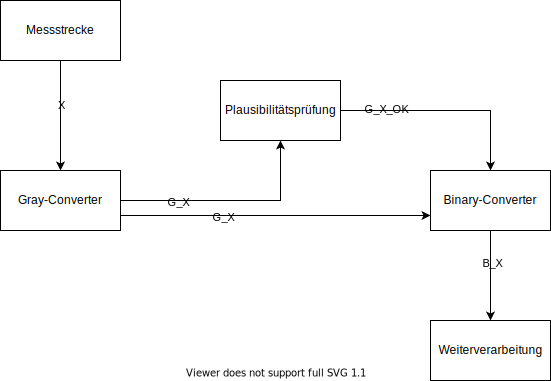
\includegraphics[width=\textwidth]{../assets/images/DIHA/blockschaltbilda.png}
  \caption{Blockschaltbild der Aufgabe A zur Plausibilitätsprüfung}
  \label{fig:blockA}
\end{figure}

\section{Lösungsidee}
\label{sec:losungsidee}
Wir wollen uns zuerst einmal anschauen, was der Gray-Code überhaupt ist, um eine Idee dafür zu bekommen, mit welchen Methoden die Aufgabe bewältigen können.


\paragraph{Hamming-Distanz}
Während bei dem in der Digitaltechnik sehr verbreitetem Binärcode die sogenannte Hamming-Distanz unterschiedlich groß sein kann, ist der Gray-Code so konzipiert, dass diese immer nur genau 1 beträgt. Die Hamming-Distanz beschreibt dabei die Distanz zwischen zwei aufeinanderfolgenden Zahlenwerten charakterisiert als die Differenz in den Ziffern der beiden Zahlen. Die Zahl $n = 3$ und zu der Zahl $n = 4$ haben die binären Darstellungen $n_{B} = 11_{(2)}$ und $n_{B}+1 = 100_{(2)}$. Die Hamming-Distanz ist hier also $3$, da sich drei Stellen der Zahl zu der nächsten ändern. Für die Messung von Messstrecken findet sich so keine einfache Methode, die Richtigkeit bzw. Plausibilität der Werte zu testen. Im Gegensatz dazu findet sich $n_{G} = 010_{(2G)}$ und $n_{G}+1 = 110_{(2G)}$ mit einer Hamming-Distanz von $1$. Hier können wir einfach überprüfen, ob der Wert, der als nächstes eingelesen wird, sich in der Hamming-Distanz um $1$ von dem vorherigen verändert hat. Wenn nicht, so stimmt die Messung nicht vollständig oder die Auflösung ist nicht hoch genug. Besonders bei Messungen von Werten, die keine allzu starken Schwankungen erlauben, ist diese Art der Plausibilitätsprüfung sehr sinnvoll.

\paragraph{Konkrete Idee}
Wie oben erwähnt, bietet es sich bei der Aufgabe an, mithilfe der Eigenschaften des Gray-Codes eine Überprüfung der Plausibilität durchzuführen. Dafür wollen nehmen wir unser Eingangssignal $G\_{X}$ und speichern dies zunächst auf ein Signal buf, um es später mit dem im nächsten Zyklus eingelesenem Eingangssignal zu vergleichen. Basierend auf dem Ergebnis der Hamming-Distanz-Berechnung setzen wir $G\_X\_OK$ also entweder auf True oder False. Das eingelesene Signal $G\_{X}$ wird das neue buf und der Prozess wiederholt sich.

\newpage

\section{Beschreibung in VHDL}
\label{sec:beschreibung-vhdl}
\begin{longlisting}
  \centering
  
  \begin{minted}{vhdl}
  library ieee;
  use ieee.std_logic_1164.all;
  use ieee.numeric_std.all;
  use ieee.math_real.all;

  entity plausible is
    port (
      G_X    : in bit_vector(9 downto 0);
      G_X_OK : out bit
    );
  end plausible;

  architecture arch of plausible is

    signal buf, plausible : bit_vector(9 downto 0);

  begin

    -- Evaluates the current signal with the buffered previous data
    eval : process begin
      wait on G_X;
      plausible <= buf xor G_X;
      buf       <= G_X;
    end process eval;

    -- Counts the differences between the evaluated signal and the buffered one
    count : process
      variable sum : integer := 0;
    begin
      wait on plausible;
      sum := 0;
      for i in 0 to 9 loop
        if plausible(i) = '1' then
          sum := sum + 1;
        end if;
      end loop;
      if sum <= 1 then
        G_X_OK <= '1';
      else
        G_X_OK <= '0';
      end if;
    end process;

  end architecture;
  \end{minted}
  \caption{Der Code für die Plausibilitätsprüfung}
  \label{fig:codeA}
\end{longlisting}
\noindent
Wir überprüfen zunächst in \textit{eval} die Hammingdistanz zwischen \textit{buf} und \textit{G\_X} und speichern dann in unserem Buffer den derzeitigen Wert von \textit{G\_X}. In \textit{count} benutzen wir eine Integervariable, um die $1$ in dem Signal \textit{plausible} zu zählen, welche das Ergebnis der Hammingdistanz enthält. Wenn dann sum über den Wert $1$ geht, dann ist das Signal nach unserem Verständnis nicht mehr plausibel. 

\newpage

\section{Simulation der Ergebnisse}
\label{sec:simul-der-ergebn}

Da wir unsere Schaltung in ModelSim simulieren, verwenden wir eine .do-Datei, um den Verlauf der Schaltung zu simulieren. Wir wollen dabei sowohl den Fall erproben, dass die Daten richtig sind, als auch, dass die Daten zuweit voneinander entfernt sind, um plausibel zu sein.

\begin{figure}[h]
  \centering
  \includegraphics[width=\textwidth]{../assets/images/DIHA/simuA.png}
  \caption{Die Simulation der Ergebnisse}
  \label{fig:simuA}
\end{figure}



\begin{longlisting}
  \centering
  \begin{minted}{vhdl}
    vsim work.plausible
    restart
    view wave
    radix bin
    add wave *


    force G_X "1010101010"
    run 20ns

    force G_X "1111111111"
    run 20ns

    force G_X "1111111110"
    run 20ns
  \end{minted}
  \caption{.do-File (Testbench) zur Simulation der Ergebnisse in \ref{fig:simuA}}
  \label{code:doA}
\end{longlisting}


\section{Fazit}
\label{sec:fazit}

Wir können anhand unserer Ergebnisse einige Dinge feststellen. Zum einen ist es wirklich erstaunlich, wie die Eigenschaften von speziellen Codes die Verarbeitung und Implementierung von bestimmten Lösungen vereinfacht. Die Logik, um eine solche Plausibilitätsprüfung durchzuführen, wenn die Eingangsdaten zum Beispiel weiterhin als Binärcode kodiert sind, wäre um einiges komplizierter und außerdem nicht wirklich effizient oder wirtschaftlich. Es bietet sich also stark an, die Möglichkeit von den verschiedenen Codes aus der Digitaltechnik einzustudieren. Es ist außerdem ersichtlich, dass sich eine Darstellung von Problemstellungen nach dem gelernten Schema anbietet. Es lässt einen stark über die einzelnen Komponenten und die Zusammenarbeit auf einem tatsächlichen FPGA-Board nachdenken.


\renewcommand{\thechapter}{B}

\chapter{Berechnung der Regelabweichung}
\label{cha:berechn-der-regel}
\newpage
\section{Aufgabe}
\label{sec:einleitung-1}

\begin{task}
  TIn der nächsten Aufgabe soll es um die Berechnung der Regelabweichung von zwei Signalen mithilfe eines Carry-Lookahead-Addierers gehen. Dabei ist unser auf Plausibilität geprüfte Signal $B\_X$ mit einem Sollwert $B\_{W}$ zu vergleichen und die Differenz auf einer bidirektionalen 10-bit breiten Busleitung auszugeben. Ebenfalls sollen die dedizierten Signale EXAKT und ZU\_KLEIN seperat je nach Ergebnis ausgegeben werden.

\end{task}


\section{Blockschaltbild}
\label{sec:blockschaltbild-1}

\begin{figure}[h]
  \centering
  \includegraphics[width=\textwidth]{../assets/images/DIHA/delta.png}
  \caption{Blockschaltbild für die Regelabweichung}
  \label{fig:blockregel}
\end{figure}


\newpage

\section{Automatengraph}
\label{sec:automatengraph}

\begin{figure}[h]
  \centering
  \includegraphics[width=\textwidth]{../assets/images/DIHA/partBauto.png}
  \caption{Der Automatengraph für die Berechnung der Regelabweichung}
  \label{fig:autopartB}
\end{figure}



\begin{table}[h]
  \centering
  \begin{tabular}{|c|c|}
    \hline
    Zustand/Signal & Erklärung \\
    \hline
    CALC & \makecell{Der CALC-Zustand stellt die durchgehende Berechnung\\ des Ergebnisses dar. Der zugehörige Übergang $CALC\in\Sigma$\\ stellt die jeweilige Beendigung des anderes Zustands dar. Im Falle\\ von ST\_DELTA z.B. das Ende von zwei Systemtakten.} \\
    \hline
    ST\_B\_X & \makecell{In diesem Zustand wird der neue Ist-Wert\\ von Bus eingelesen. Dieses wird von dem Steuersignal ST\_B\_X eingeleitet.}\\
    \hline
    ST\_B\_W & \makecell{In diesem Zustand wird der neue Soll-Wert von Bus eingelesen.\\ Dieses wird von dem Steuersignal ST\_B\_W eingeleitet.}\\
    \hline
    ST\_DELTA & \makecell{In diesem Zustand wird das Ergebnis auf dem Bus ausgegeben.\\ Dabei gibt das Signal ST\_DELTA das Signal, den Bus zwei Systemtakte lang \\ mit dem Ergebnis zu beschreiben.} \\
    \hline
  \end{tabular}
  \caption{Erklärung der einzelnen Zustände und Übergänge}
  \label{tab:state}
\end{table}


\section{Lösungsidee}
\label{sec:losungsidee-1}

Wir wollen uns nun einmal anschauen, mit welchen Mitteln wir unser Ziel erreichen können.

\subsection{Carry-Lookahead-Addierer}
\label{sec:carry-look-addi}

Bei dem Carry-Lookahead-Addierer, den wir für unsere Berechnung der Regelabweichung verwenden wollen, handelt sich um eine Weiterentwicklung des Carry-Ripple-Addierers. Hier werden also nicht einfach nur mehrere Volladdierer miteinander so verschaltet, dass mehrere Bit breite Signale miteinander addiert werden können, sondern es gibt ein komplizierteres System, um die Übertrage der Volladdierer zu bestimmen. Fundamental für diese Überlegung sind die Konzepte von Generate, Propagate und Absorb.\cite{skript}

\paragraph{Generate}

Bei Generate handelt sich um ein logisches Prädikat, welches wir im Folgenden durch $G(A, B)$ bezeichnen möchten mit $G(A,B) = A \cdot B$, wobei $\cdot$ das logische Und darstellt. Wir sagen also, dass zwei Ziffern genau dann generieren, wenn die beiden Ziffern immer einen Übertrag bilden und dieser nicht abhängig ist, ob ein weiterer Übertrag auf die Ziffern hinzuaddiert werden.

\paragraph{Propagate}

Bei Propagate handelt es sich ebenfalls um ein logisches Prädikat, welches wir im Folgenden mit $P(A,B) = A + B$ bezeichnen, wobei $+$ das logische Oder darstellt. Wir sagen also, dass zwei Ziffern genau dann propagieren, wenn die beiden Ziffern nur dann einen Übertrag bilden, wenn ein weiterer Übertrag von der Berechnung vorher kommt.

\paragraph{Absorb}

Wir wollen im folgenden Absorb als denjenigen Zustand definieren, der einen Übertrag von der vorherigen Berechnung absorbieren würde, dabei allerdings keinen Übertrag generiert. Mit $A(A,B) = \not(A + B)$ definieren wir einen Zustand, der das Gegenteil von Propagate darstellt und nur dann wahr ist, wenn beide Ziffern (im Falle einer binären Addition) $0$ sind.

\subsection{Zweier Komplement}
\label{sec:zweier-komplement}

Wenn wir die Differenz von zwei binären Zahlen berechnen wollen, müssen wir eine der beiden, da unser Carry-Lookahead-Addierer eigentlich nur Addition beherrscht, in ein anderes Format umwandeln, um eine Differenz berechnen zu können. Wir entscheiden uns hier für das Zweier Komplement, um aus einer der beiden Signalen, die eine binäre Zahl darstellen, eine negative Zahl zu machen, und diese dann zu addieren.

Bei der Umwandlung gehen wir dabei nach folgendem Schema vor:

\begin{enumerate}
  \item Wir invertieren alle weiteren Bits, alle $1$ werden zu $0$ und umgekehrt.
  \item Das Most-Significant-Bit stellt im zweier Komplement das Vorzeichen dar.
  \item Zum Schluss addieren wir auf die Zahl eine $1$, unsere Zahl ist damit umgewandelt.
\end{enumerate}

Umgekehrt setzen wir die Schritte einfach erneut ein, wir invertieren also alle Stellen und addieren dann eine $1$ auf die derzeitige Zahl. Wir erhalten genau die Zahl, mit der wir begonnen haben.

\subsection{Taktsynchronität}
\label{sec:taktsynchronitat}

Wir müssen uns nun noch mit der Anforderung an unsere Lösung beschäftigen, taktsynchron und in Harmonie mit dem Busarbiter zu funktionieren. Dafür wollen wir in unserer Beschreibung mit VHDL eine Top-Level-Komponente einrichten, die sich um genau diese Anforderungen kümmert. Wir nennen diese comparator. Sie wird sich mithilfe des Moore-Automatengraphs durch die einzelnen Zustände des Automaten arbeiten und die entsprechenden Daten aus dem bidirektionalen Bus einlesen, weiterverarbeiten und dann auf dem gleichen Bus ausgeben. 
\newpage

\section{Beschreibung in VHDL}
\label{sec:beschreibung-vhdl-1}

\subsection{Volladdierer}

\begin{longlisting}
  \centering
  \begin{minted}{vhdl}
    library ieee;
    use ieee.std_logic_1164.all;
    use ieee.numeric_std.all;
    use ieee.math_real.all;
    
    
    entity fulladder is
      port (
        a    : in bit;
        b    : in bit;
        cin  : in bit;
        S    : out std_logic;
        cout : out bit
      );
    end entity fulladder;
    
    architecture behav of fulladder is
    
    begin
      S    <= To_STDULOGIC(a xor b xor cin);
      cout <= (a and b) or (cin and a) or (cin and b);
    end architecture;
  \end{minted}
  \caption{Der Volladdierer als Baustein des Carry-Lookahead-Addierers}
  \label{code:fulladder}
\end{longlisting}
\vspace*{1em}
\noindent
Der Volladdierer ist schon aus der Vorlesung bekannt und wurde in vergangenen Praktika bereits verwendet. Dabei ist allerdings zu bemerken, dass hier bereits Verzögerungen und eine Umwandlung von Bit zu STD\_LOGIC vorgenommen wurde. Der Hintergrund ist die anschließende Umwandlung des Signals mittels der signed und abs Funktionen der Standardbibliothek IEEE.

\newpage

\subsection{Carry-Lookahead-Addierer}
\begin{longlisting}
  \centering
  \begin{minted}{vhdl}
    library ieee;
    use ieee.std_logic_1164.all;
    use ieee.numeric_std.all;
    
    entity carrylookahead is
      port (
        add1   : in bit_vector(9 downto 0);
        add2   : in bit_vector(9 downto 0);
        sign   : out std_logic;
        result : out std_logic_vector(8 downto 0)
      );
    end entity;
    
    architecture behav of carrylookahead is
      component fulladder
        port (
          a    : in bit;
          b    : in bit;
          cin  : in bit;
          S    : out std_logic;
          cout : out bit
        );
      end component;
      signal carry : bit_vector(10 downto 0);
      signal sum   : std_logic_vector(9 downto 0);
      signal gen   : bit_vector(10 downto 0);
      signal prop  : bit_vector(10 downto 0);
    begin
      clahgen : for i in 0 to 9 generate
        fulladder_inst : fulladder
        port map(
          a    => add1(i),
          b    => add2(i),
          cin  => carry(i),
          S    => sum(i),
          cout => open
        );
      end generate;
    
      genprop : for j in 0 to 9 generate
        gen(j)       <= add1(j) and add2(j);
        prop(j)      <= add1(j) or add2(j);
        carry(j + 1) <= gen(j) or (prop(j) and carry(j));
      end generate;

      carry(0) <= '1';
      sign     <= sum(9);
      result   <= std_logic_vector(abs(signed(sum(result'range))));
    end architecture;    
  \end{minted}
  \caption{Der Carry-Lookahead-Addierer, dabei wird das Ergebnis automatisch in das gewünschte Format geschrieben}
  \label{code:cla}
  
\end{longlisting}
\newpage
%\vspace*{1em}
\noindent
Die Logik des Carry-Lookahead-Addierers, die wir in \ref{sec:carry-look-addi} bereits beschrieben haben, wird nun mittels einiger For-Generate-Statements verwirklicht. Es werden also entsprechend viele Volladdierer, sowie die Logik für Generate, Propagate und Carry-Over generiert und diese dann zum Schluss mittels $std\_logic\_vector(abs(signed(sum(result'range))))$ in den entsprechenden Betrag umgewandelt wird. Das Vorzeichen wird in \textit{sign} gespeichert.\cite{vhdlwhiz}\cite{nandland}

\newpage
\subsection{Substractor}

\begin{longlisting}
  \centering
  \begin{minted}{vhdl}
    library ieee;
    use ieee.std_logic_1164.all;
    use ieee.numeric_std.all;
    use ieee.math_real.all;
    entity subtractor is
      port (
        B_X   : in std_logic_vector(9 downto 0);
        B_W   : in std_logic_vector(9 downto 0);
        DELTA : out std_logic_vector(9 downto 0)
      );
    end entity subtractor;
    
    architecture behav of subtractor is
      component carrylookahead is
        port (
          add1   : in bit_vector(9 downto 0);
          add2   : in bit_vector(9 downto 0);
          sign   : out std_logic;
          result : out std_logic_vector(8 downto 0)
        );
      end component;
    
      signal TC_B_W   : bit_vector(9 downto 0);
      signal sA       : bit_vector(9 downto 0);
      signal sR       : std_logic_vector(8 downto 0);
      signal signedBX : std_logic;
    
    begin
    
      cla : carrylookahead
      port map(
        add1   => sA,
        add2   => TC_B_W,
        sign   => signedBX,
        result => sR
      );
      sA     <= to_bitvector(B_X);
      TC_B_W <= not(to_bitvector(B_W));
      DELTA  <= signedBX & sR;
    end architecture;
  \end{minted}
  \caption{Der Subtractor, der die Verarbeitung der Werte aus dem Vergleicher mit dem Carry-Lookahead-Addierer übernimmt}
  \label{code:sub}
\end{longlisting}

\noindent
Der Substractor behandelt nun implizit die Umrechnung des Sollwerts in das Zweierkomplement, um eine Subtraktion der beide Signale durchführen zu können. Dabei wird das Signal \textit{TC\_B\_W} zunächst einfach konvertiert. Durch das $Cin_0$ des Carry-Lookahead-Addierers, welches wir in der Datei auf $1$ gesetzt haben, ist das Addieren der $1$ zur Umwandlung in das Zweierkomplement auch gegeben. Zum Schluss wird dann \textit{DELTA} durch eine Konkatenation, die in VHDL über \& passiert, des Vorzeichens und des Betrags aus dem Ergebnis des Carry-Lookahead-Addierers gebildet.\cite{DIG} 


\newpage
\subsection{Vergleicher}

\begin{longlisting}
  \centering
  \begin{minted}{vhdl}
    library ieee;
    use ieee.std_logic_1164.all;
    use ieee.numeric_std.all;
    use ieee.math_real.all;
    
    entity comparator is
      port (
        clk      : in std_logic;
        reset    : in std_logic;
        io       : inout std_logic_vector(9 downto 0) := "ZZZZZZZZZZ";
        ST_B_X   : in bit;
        ST_B_W   : in bit;
        ST_DELTA : in bit;
        EXAKT    : out bit;
        ZU_KLEIN : out bit
      );
    end entity comparator;
    
    architecture rtl of comparator is
      component subtractor is
        port (
          B_X   : in std_logic_vector(9 downto 0);
          B_W   : in std_logic_vector(9 downto 0);
          DELTA : out std_logic_vector(9 downto 0)
        );
      end component;
    
      signal result : std_logic_vector(9 downto 0);
      type statetype is (reading_BX, reading_BW, calculating, output);
      signal X, W       : std_logic_vector(9 downto 0) := "0000000000";
      signal state      : statetype                    := calculating;
      signal next_state : statetype                    := calculating;
    begin
    
      sub : subtractor
      port map(
        B_X   => X,
        B_W   => W,
        DELTA => result
      );
    
      WR : process (state, clk, ST_DELTA)
      begin
        if state = output and clk'event and clk = '1' then
          io <= result;
        elsif state = calculating and clk'event and clk = '1' then
          io <= (others => 'Z');
        end if;
        if result(9) = '1' then
          ZU_KLEIN <= '1';
        elsif X = W then
          EXAKT <= '1';
        else
          ZU_KLEIN <= '0';
          EXAKT    <= '0';
        end if;
      end process;
    
      RD : process (io, ST_B_X, clk)
      begin
        if state = reading_BX and clk'event and clk = '1' then
          X <= io;
        elsif state = reading_BW and clk'event and clk = '1' then
          W <= io;
        end if;
      end process;
    
      SW : process (reset, clk)
      begin
        if clk'event and clk = '1' and reset = '1' then
          state <= calculating;
        elsif clk'event then
          state <= next_state;
        end if;
      end process;
    
      SN : process (ST_B_W, ST_B_X, ST_DELTA, clk)
        variable counter : integer := 0;
      begin
        case state is
          when calculating =>
            io <= "ZZZZZZZZZZ";
            if ST_B_X = '1' then
              next_state <= reading_BX;
            elsif ST_B_W = '1' then
              next_state <= reading_BW;
            elsif ST_DELTA = '1' then
              next_state <= output;
            end if;
          when reading_BX =>
            if ST_B_X = '0' then
              next_state <= calculating;
            elsif ST_B_W = '1' then
              next_state <= reading_BW;
            elsif ST_DELTA = '1' then
              next_state <= output;
            end if;
          when reading_BW =>
            if ST_B_W = '0' then
              next_state <= calculating;
            elsif ST_B_X = '1' then
              next_state <= reading_BX;
            elsif ST_DELTA = '1' then
              next_state <= output;
            end if;
          when output =>
            if clk'event and clk = '1' then
              counter := counter + 1;
              if clk'event and clk = '1' and counter = 2 then
                next_state <= calculating;
                counter := 0;
              end if;
            end if;
        end case;
      end process;
    end architecture;
  \end{minted}
  \caption{Der Hauptprozess, der den Zugriff auf den Bus (io) übernimmt.}
  \label{code:comp}
\end{longlisting}

\noindent
In diesem Prozess behandeln wir, wie wir die Taktsynchronität, wir in \ref{sec:taktsynchronitat} schon angesprochen haben, umsetzen wollen. Wir verwenden den in \ref{sec:automatengraph} erstellten Graphen, um im Prozess \textit{SN} die Bedingungen für das Ändern des Zustandes wählen. Über das Signal \textit{io}, was den Bus darstellt, werden in den richtigen Momenten die Werte eingelesen. Der Prozess \textit{SW} wechselt vom \textit{state} in den \textit{next\_state}, und zwar immer auf dem Ändern des Clocksignals. Hier wird außerdem noch der Reset eingelesen und verarbeitet. Der Prozess \textit{WR} schreibt, sollte der Zustand auf \textit{output} sein, das Ergebnis des \textit{subtractors} auf den Bus, ansonsten wird dieser auf hochohmig gelegt. Der letzte Prozess \textit{RD} liest bei gegebenen Zustand den des Busses aus. 

\section{Simulation der Ergebnisse}
\label{sec:simul-der-ergebn-1}

\begin{figure}[h]
  \centering
  \includegraphics[width=\textwidth]{../assets/images/DIHA/simuB.png}
  \caption{Simulation der Beschreibung in VHDL}
  \label{fig:simuB}
\end{figure}

\noindent
Wir erkennen auf der Abbildung, dass wir eine relativ gute Lösung finden konnten, die mit unseren Wünschen und Anforderungen an unser System übereinstimmen. Wir lesen zunächst den Sollwert B\_W nach dem Steuersignal ST\_B\_W ein, gefolgt von dem Ist-Wert B\_X über das ST\_B\_X-Signal. Es wird über unser Substractor-Component, der den Carry-Lookahead-Addierer enthält, ein Ergebnis in unseren result-Buffer geschrieben, der dann zwei Systemtakte lang auf der bidirektionalen Busleitung io ausgegeben wird. Diese wird zwischen den Operationen, und so auch nach der Ausgabe des Ergebnisses, wieder hochohmig (dargestellt durch die blaue Linie). Auch unser Ergebnis von $16_{(10)} = 0000010000_{(2)}$, welches Sie aus der Distanz des Sollwerts $B\_W = -15_{(10)} = 1111110001_{2}$ zu dem Ist-Wert $B\_X = 1_{(10)} = 0000000001_{(2)}$ ergibt.

\newpage 

\begin{longlisting}
  \begin{minted}{vhdl}
  vsim work.comparator
  restart
  view wave
  radix bin
  add wave *

  force clk 0,1 10ns -r 20ns

  force reset 0
  force ST_B_W 0
  force ST_B_X 0
  force ST_DELTA 0
  run 50ns

  force ST_B_W 1
  force io "1111110001"
  run 10ns

  force ST_B_W 0
  run 10ns


  force ST_B_X 1
  force io "0000000001"
  run 10ns

  force ST_B_X 0
  run 10ns

  noforce io
  force ST_B_X 0
  force ST_DELTA 1
  run 100ns
  \end{minted}
  \caption{.do-File (Testbench) für die Simulation der Ergebnisse in \ref{fig:simuB}}
  \label{code:doB}
\end{longlisting}


\subsection{Kritischer Pfad}

Der kritische Pfad eines Systems beschreibt denjenigen Pfad eines Signals, welcher die längste Verzögerung von Eingang zu Ausgang bietet. So können beispielsweise große Zahlen in einem Carry-Ripple-Addierer zu größerer Berechnungszeit führen. Der kritische Pfad führt also durch alle Überträge hindurch. Wir haben bei uns, durch den Carry-Lookahead-Addierer nur noch die Verzögerung der Berechnung der Summe im Volladdierer selbst. Wir simulieren hierbei Verzögerung über \textit{after x ns}. Die Umwandlung im CLA und die Berechnung des Carryoverbits durch Generate und Propagate werden auch mit entsprechenden Werten versehen. Allerdings ist der kritische Pfad, den es zu bestimmen gilt, lediglich von der Berechnung selbst abhängig. Wir bekommen mit den Verzögerungen bei unserer Testberechnung eine Verzögerung von $12ns$, den kritischen Pfad konnten wir mit einer pauschalen Verarbeitungszeit der übrigen Schaltungselemente mit $52ns$ mit $\Delta t_g = \Delta t_b + \Delta t_v = 12ns + 40ns = 52ns$ bestimmen. Eine maximale Taktfrequenz, ergibt sich dann mit $f = \frac{1}{\Delta t_g} = \frac{1}{52ns} = 19,23MHz$ bestimmen.

\begin{figure}[h]
  \centering
  \includegraphics[width=\textwidth]{../assets/images/DIHA/simuBtimev2.PNG}
  \caption{Die Berechnung der Berechnungsverzögerung mithilfe von ModelSim}
  \label{fig:simuBtime}
\end{figure}




\section{Fazit}
\label{sec:fazit-1}

Was sich bei dieser Aufgabe als ein extrem prägnantes und sehr hilfreiches Analysewerkzeug entpuppt hat, ist die Darstellung der Zustände innerhalb eines Moore-Automaten, da sich darüber analog die Verarbeitung der Steuersignale, der Inputs und der Outputs ergeben hat. Eine Simulation eines solchen Automaten, was wir bereits im dritten Praktikum erfolgreich getan haben und uns auch in der Vorlesung angeschaut haben, hat hier die Vorgehensweise extrem linear und einfach gestaltet. Eine Umwandlung der Werte in das Zweierkomplement, eine Erweiterung des bereits verwendeten Carry-Ripple-Addierers zum Carry-Lookahead-Addierers und eine sinnvolle Verwendung bereits gelernter Konzepte hat den Rest der Aufgaben ausgemacht. Ich konnte hier allerdings Lösungen aus der Literatur, der Vorlesung und des Internets verwenden, um für alle weiteren Probleme eine gute Herangehensweise zu finden.


\renewcommand{\thechapter}{C}

\bibliographystyle{alpha}
\bibliography{DIHA}{}

\end{document}
%%% Local Variables:
%%% LaTeX-command: "latex -shell-escape"
%%% End:
